\documentclass[12pt]{article}


\usepackage[utf8]{inputenc}
\usepackage[a4paper,top=3cm,bottom=2cm,left=3cm,right=3cm,marginparwidth=1.75cm]{geometry}
\usepackage[nodayofweek]{datetime}
\usepackage{tabularx}
\usepackage[small]{titlesec}
\usepackage{graphicx}
\usepackage{tabularx}

\newcolumntype{L}[1]{>{\raggedright\arraybackslash}p{#1}}
\newcolumntype{C}[1]{>{\centering\arraybackslash}p{#1}}
\newcolumntype{R}[1]{>{\raggedleft\arraybackslash}p{#1}}

\begin{document}

\begin{titlepage}
    \begin{center}
        \huge{\bfseries  Tribhuvan University}\\
        \Large{Institute of Engineering}\\
        \huge{ \bfseries  Pulchowk Campus}\\[3.2cm]


        \textsc{\Large Internet and Intranet}\\[-0.5cm]
        \line(1,0){400}\\
        \huge{\bfseries Lab 2}\\
        \large{Apache Web Server configuration on Docker
        container}
        \line(1,0){400}\\


        \textsc{\Large Submitted by:}\\
        \Large Bishal Katuwal\\ \large 075BCT028\\    [0.85cm]

        \textsc{\Large Submitted to:}\\\
        \large Department of Electronics and Computer Engineering\\Pulchowk Campus\\    [0.85cm]
        
        \textsc{\Large Submitted on:}\\
        \today
        
    \end{center}
\end{titlepage}
\pagebreak
% ===============================================================
\paragraph{\Large Title\\}
Apache Web Server
Configuration on Docker
container

\paragraph{Background Theory\\}
The Apache HTTP Server, commonly referred to as Apache, is a free and open-source web server software. It is one of the most widely-used web servers in the world and is developed and maintained by the Apache Software Foundation. Apache is known for its stability, security, and flexibility, making it a popular choice for hosting websites and web applications.

Apache can be used on a variety of operating systems, including Windows, Linux, and macOS. It supports many different technologies and protocols, such as HTTP, HTTPS, and various scripting languages like PHP, Perl, and Python. Additionally, it can be extended using various modules, such as mod\textunderscore rewrite for URL rewriting, mod\textunderscore ssl for HTTPS support, and mod\textunderscore proxy for reverse proxying.
Apache can be configured using a configuration file called httpd.conf, which contains various settings that control the behavior of the web server. This file can be used to set up virtual hosts, configure security settings, and configure other server options.

\paragraph{Activity}
\section{Docker Installation}
\begin{enumerate}
    \item Updated system packages.
    \begin{verbatim}
        sudo apt update
    \end{verbatim}
    \item Installed dockerpackage.
    \begin{verbatim}
        sudo apt install docker 
    \end{verbatim}
    \item Checked the version of docker.
    \begin{verbatim}
        docker --version
    \end{verbatim}
\end{enumerate}
\begin{figure}[h!]
    \centering
    
\includegraphics[scale = 0.70]{Images/docker_version.PNG}
    \caption{Docker installation}
\end{figure}
\section{Running Docker Image}
\begin{enumerate}
    \item Pulled httpd image
    \begin{verbatim}
        sudo docker pull httpd
    \end{verbatim}
    \item Created a html page to be served with apache web server
    \begin{verbatim}
        <!DOCTYPE html>
        <html lang="en">
        <head>
            <title>Test Server</title>
        </head>
        <body>
            Hello.
        </body>
        </html>
    \end{verbatim}
    \begin{figure}[h!]
        \centering
        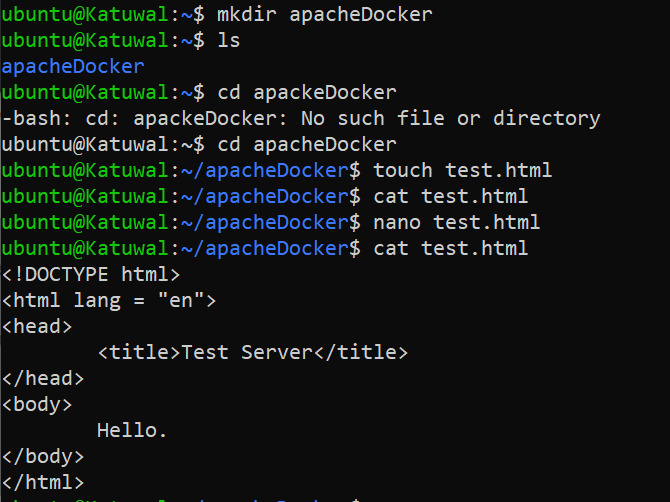
\includegraphics{Images/apacheHTML.PNG}
        \caption{HTML file}
    \end{figure}

    \item Launched the docker container.
    \begin{verbatim}
sudo docker images
docker run -dit --name my-apache-app -p 8080:80 -v "$PWD":/usr/local/
        apache2/htdocs/ httpd
    \end{verbatim}
    \begin{figure}[h!]
        \centering
        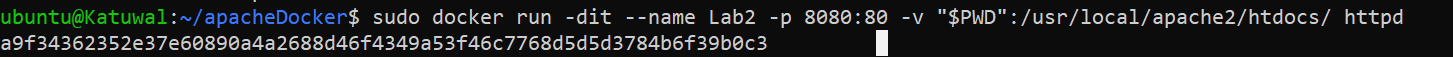
\includegraphics[scale = 0.50]{Images/docker_run.PNG}
        \caption{Docker run}
    \end{figure}
\end{enumerate}

\section{Test server}
\begin{figure}[h!]
    \centering
    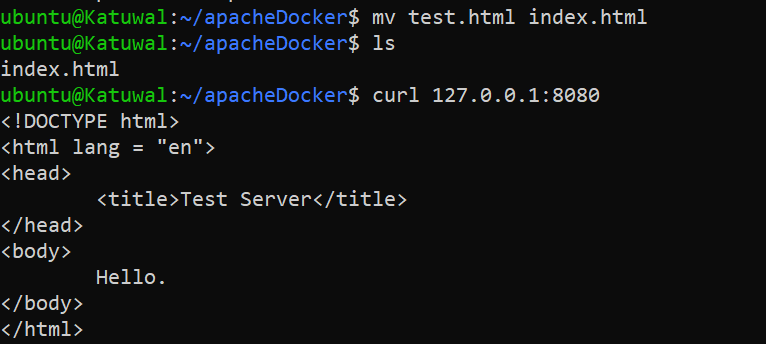
\includegraphics[scale = 0.70]{Images/serverRun.PNG}
    \caption{Docker test}
\end{figure}
\paragraph{Conclusion\\}
In this report, we have discussed the basic steps for Apache Web Server configuration on Docker
container on Linux operating systems. 
The process of configuring Apache webserver in docker contaimer involves 
installing the docker software, 
configuring the apache image, and 
testing the server to ensure it is working properly.

\end{document}